\section{Flows}
\label{sec:flows}
\index{Automation!flows|see {Flows}}\index{Flows}
Flows provide a no-code method for developing advanced automations in Gravwell. A flow consists of one of more \emph{nodes}; each node performs a single action and passes the results (if any) on to the next node(s). By wiring together nodes in a drag-and-drop user interface, users can:

\begin{itemize}
\tightlist
\item Run queries
\item Generate PDF reports
\item Send emails
\item Fire off Slack and MS Teams messages
\item Re-ingest alerts
\item etc.
\end{itemize}

\subsection{Flow Concepts}
\label{sec:flow-concepts}

Flows are automations, meaning they are normally executed on a user-specified schedule by the search agent. They can also be run manually through the user interface. The basic process of flow development is:

\begin{enumerate}
\item Create a new flow
\item Instantiate nodes in the flow and connect them together
\item Configure nodes
\item Test the flow with debug runs
\item Deploy the flow by setting a schedule \& enabling scheduled execution
\end{enumerate}

\subsubsection{Nodes}
\index{Flows!nodes}
A flow is a collection of \emph{nodes}, linked together to define an order of execution. Each node does a single task, such as running a query or sending an email. Figure \ref{fig:nodes} shows a simple flow of three nodes; the leftmost node runs a Gravwell query, then the middle node formats the results of that query into a PDF document, and finally the rightmost node sends that PDF document as an email attachment.

\begin{figure}
	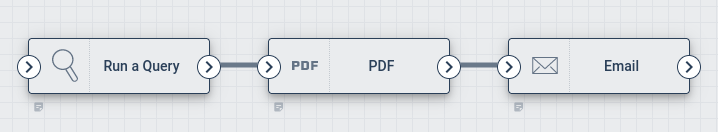
\includegraphics[width=0.7\linewidth]{images/nodes.png}
	\caption{A simple flow with three nodes.}
	\label{fig:nodes}
\end{figure}

All nodes have a single output socket. Most have only a single input socket, but some nodes which merge \emph{payloads} (see below) have multiple input sockets. One node's output socket may be connected to the \emph{inputs} of multiple other nodes, but each input socket can only take one connection.

\subsubsection{Payloads}
\index{Flows!payloads}
\emph{Payloads} are collections of data passed from node to node, representing the state of execution. For instance, the ``Run a Query'' node will insert an item named ``search'' into the payload, containing things like the query results and metadata about the search. The PDF node can \emph{read} that ``search'' item, format it into a nice PDF document, and insert the PDF file back into the payload with a name like ``gravwell.pdf''. Then the Email node can be configured to attach ``gravwell.pdf'' to the outgoing email.

Most nodes receive a single incoming payload through a single \emph{input} socket, then pass a single outgoing payload via the \emph{output} socket. In most cases, the outgoing payload will be a modified version of the incoming payload.

The \emph{merge} nodes are exceptions to this general rule. The Stack Merge and Nest Merge nodes take multiple incoming payloads (via multiple input sockets) and merge them into a single output. See Section \ref{sec:nodes} for more detailed descriptions of these nodes.

\subsubsection{Execution order}

Nodes are always executed one at a time. A node can be executed if all nodes upstream of it (its \emph{dependencies}) have executed. If multiple nodes are ready to execute, one will be chosen at random. In Figure \ref{fig:execution}, both the ``Run a Query'' node and the ``HTTP'' node are candidates to run first. After the Query node finishes, the If node can execute; when it is done, the Slack Message node may run. We say that the ``If'' node is \emph{downstream} of the Query node, and the Slack node is \emph{downstream} of both the If and Query nodes.

\begin{figure}
	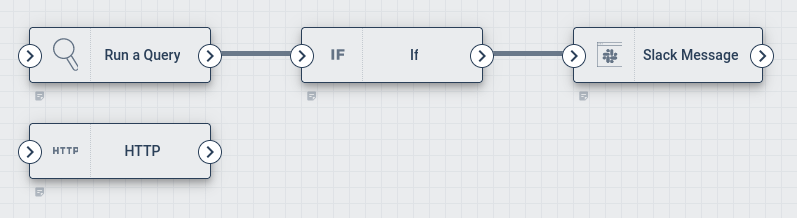
\includegraphics[width=0.7\linewidth]{images/execution.png}
	\caption{An illustration of execution order.}
	\label{fig:execution}
\end{figure}

Note that some nodes may block execution of downstream nodes. The \code{If} node is configured with a boolean logic expression; if that expression evaluates to \emph{false}, none of the If node's downstream nodes are executed. Nodes which can block downstream execution will always have a note to that effect in the online documentation.

\subsection{The Flow Editor}
\index{GUI!flow editor}
Flows are created using the flow editor. Although the Gravwell flow editor can be intimidating at first glance, a few minutes' worth of experimentation and exploration should be enough to get started building flows. This section will go through the various components of the UI, explaining each component.

Note: If you're not yet familiar with the basic components of a flow (nodes, sockets, payloads), refer to Section \ref{sec:flow-concepts} for an overview.

You can access the flow editor from the Query \& Dev Studio interface, found in the Main Menu. Select ``Flows'' from the left-hand side, as shown in Figure \ref{fig:dev-studio-newflow}. From there, you can either start a new blank flow (``Start a New Flow'') or instantiate one of the ``starter flows'' provided by Gravwell.

\begin{figure}
	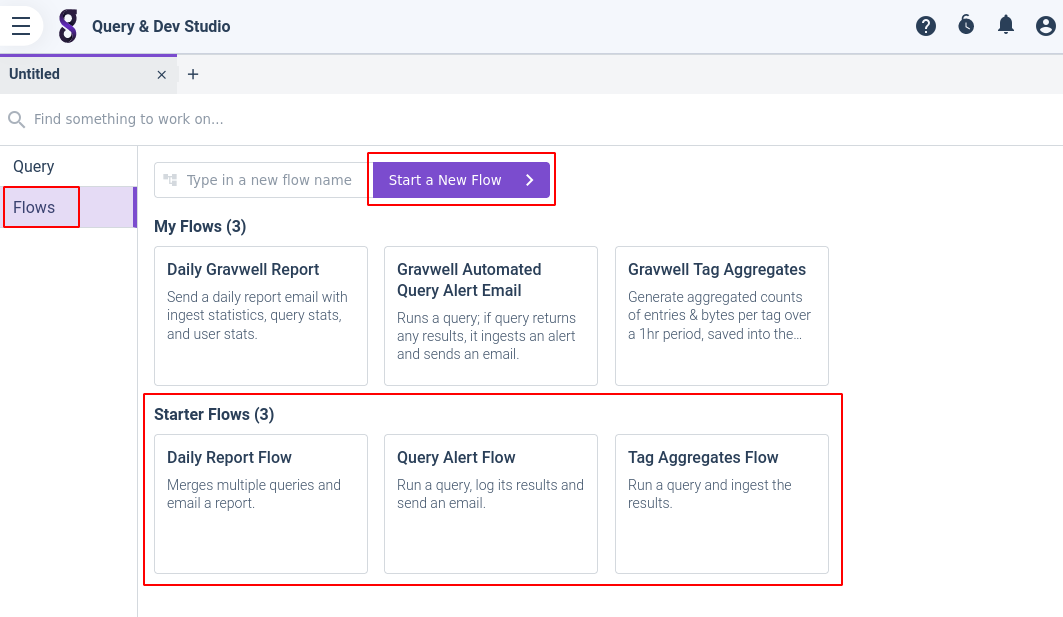
\includegraphics[width=0.8\linewidth]{images/dev-studio-newflow.png}
	\caption{Flows in the Query Studio}
	\label{fig:dev-studio-newflow}
\end{figure}

Selecting either option will take you into the flow editor, the parts of which are marked in Figure \ref{fig:flow-editor}. The \emph{palette} provides a list of available nodes, which can be dragged out into the \emph{canvas}. The \emph{console} provides information about problems with the flow and output from any test runs.

\begin{figure}
	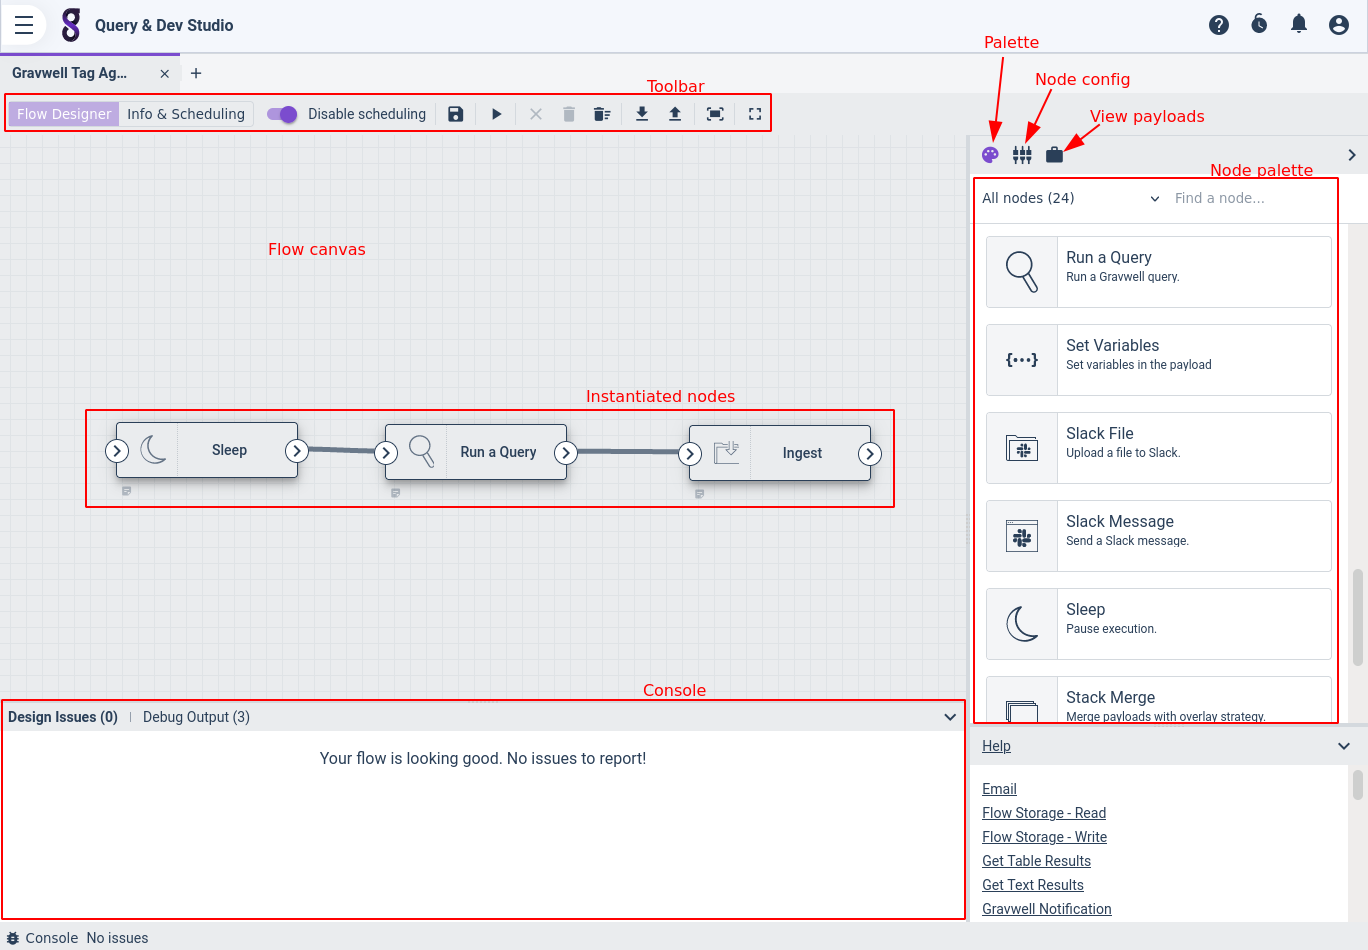
\includegraphics[width=0.85\linewidth]{images/flow-editor.png}
	\caption{Parts of the Flow Editor.}
	\label{fig:flow-editor}
\end{figure}

Nodes are instantiated by dragging them from the palette onto the canvas. Once on the canvas, node input and output sockets can be connected, nodes can be re-arranged, etc. Note that the scroll wheel can be used to zoom in and out of the canvas view.

The toolbar contains buttons for quick access to editor functionality. From left to right:

\begin{itemize}
\item Flow Designer: shows the flow canvas (default view).
\item Info \& Scheduling: shows options to set flow name, description, scheduling, sharing, etc.
\item Disable scheduling: toggle to quickly enable/disable automatic execution of the flow.
\item Save: save the flow.
\item Debug: run the flow
\item Clear selection: deselects any currently-selected node.
\item Delete: delete the selected node.
\item Delete all: delete all nodes (requires confirmation).
\item Export flow: download the flow specification, for backup or sharing.
\item Import flow: upload a previously-exported flow spec.
\item Fit all nodes on screen: zoom \& center the canvas so that \emph{all} nodes are visible.
\item Fullscreen: puts the editor into fullscreen mode.
\end{itemize}

\subsubsection{Configuring Nodes}

Once a node has been instantiated by dragging it from the palette to the canvas, it must be configured. Clicking on the node will bring up the configuration pane as seen in Figure \ref{fig:node-config}.

\begin{figure}
	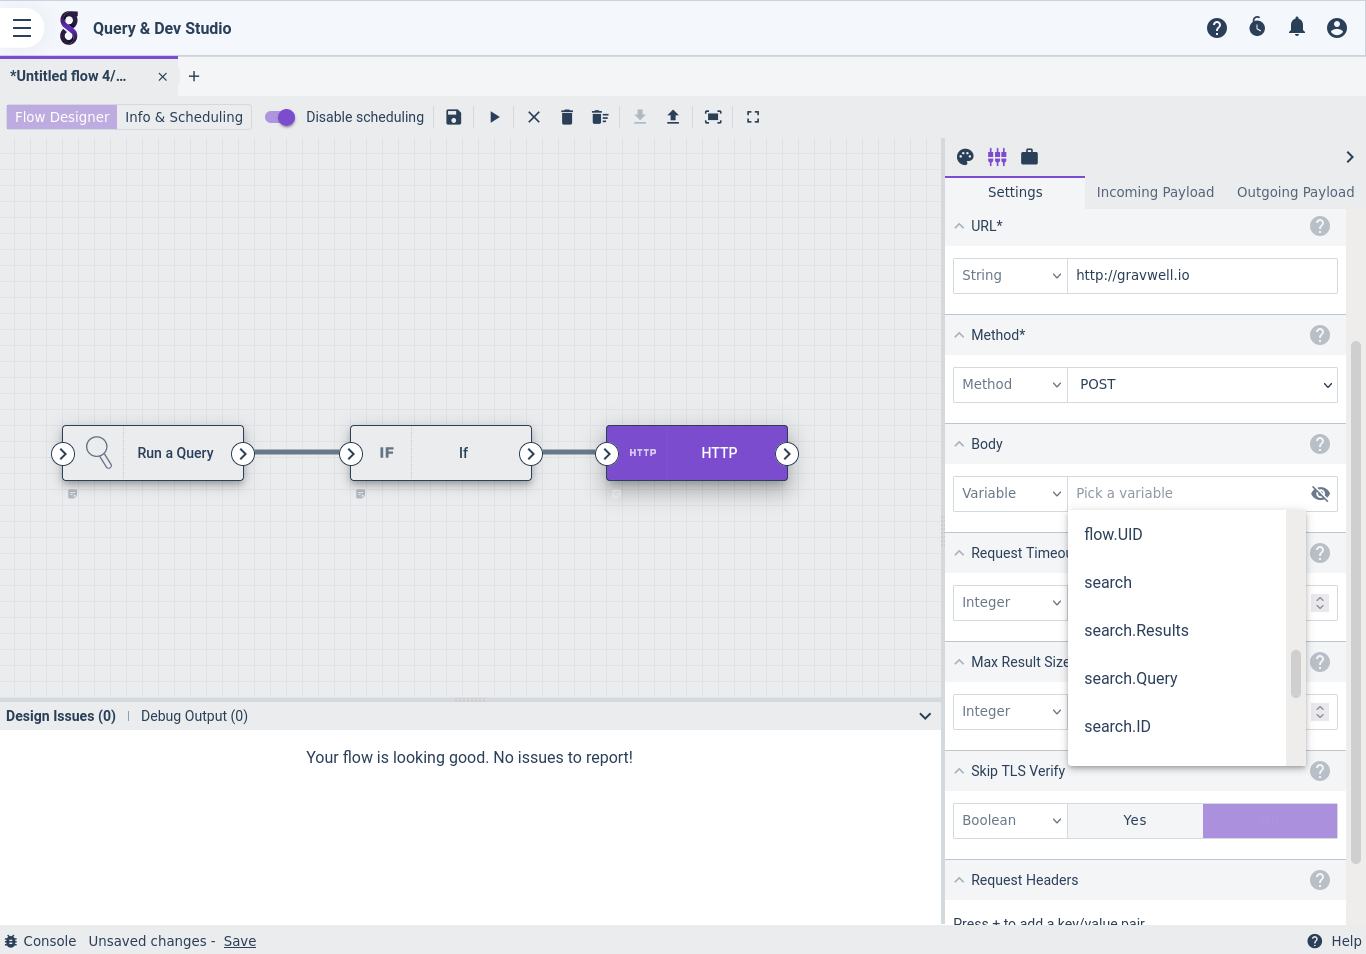
\includegraphics[width=0.85\linewidth]{images/node-config.png}
	\caption{Configuring a node.}
	\label{fig:node-config}
\end{figure}

The HTTP node shown in Figure \ref{fig:node-config} is a particularly complex node with many config options, which serves well for demonstration. Note that the URL and Method fields are marked with an asterisk, indicating that they are required. Note also the drop-down menus for each config option; these allow you to change between entering a constant value (e.g. the string ``http://gravwell.io'' in the URL config) or selecting a value from the payload as shown with the Body config.


If a node is misconfigured, the console will display a list of problems. In Figure \ref{fig:parse-errors}, we see that the Email node has several config options which are not yet set. As those options are populated, the errors will go away.

\begin{figure}
	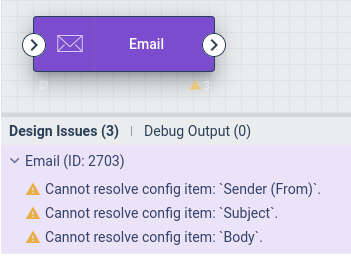
\includegraphics[width=0.85\linewidth]{images/parse-errors.png}
	\caption{Parse errors.}
	\label{fig:parse-errors}
\end{figure}

Note: You can return to the palette view at any time by clicking the palette icon above the configuration pane.

\subsubsection{Debugging}

Once a flow has been designed and configured, it can be debugged. This will signal the search agent component that it should try executing the flow. To start a debug run, click the ``Run flow and debug'' button (the ``play button'') in the toolbar. The user interface will then wait for the search agent to complete its run.

Once the run is complete, the console will have detailed execution information for each node in the ``Debug Output'' pane. The nodes are listed in order of execution. Clicking on a node in the debug output will bring up a pane showing that node's log output and the actual contents of that node's output payload. In Figure \ref{fig:if-payload}, we can see that the If node received a payload where \code{search.Count} was ``10'', meaning the If node's boolean statement evaluated to true and the HTTP node was allowed to execute:

\begin{figure}
	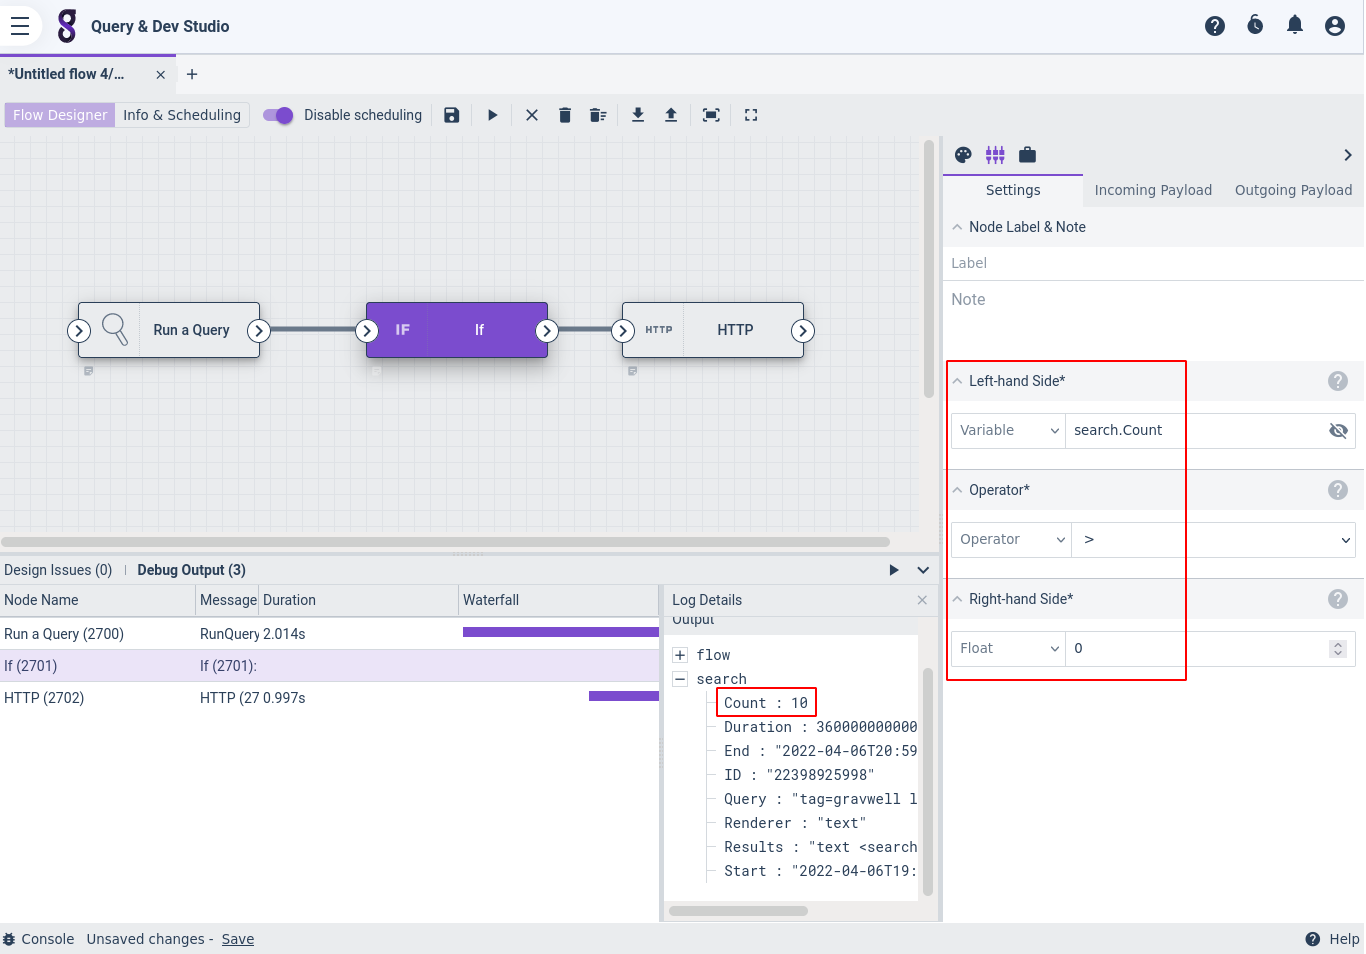
\includegraphics[width=0.85\linewidth]{images/if-payload.png}
	\caption{Node payload showing If node payload.}
	\label{fig:if-payload}
\end{figure}

If we modify the If node's config so the statement is \code{search.Count <= 0} and re-run the flow, we'll see that it now evaluates to false and the HTTP node does not execute (as seen by the empty ``Message'' column in the Debug Output pane), as shown in Figure \ref{fig:if-false}

\begin{figure}
	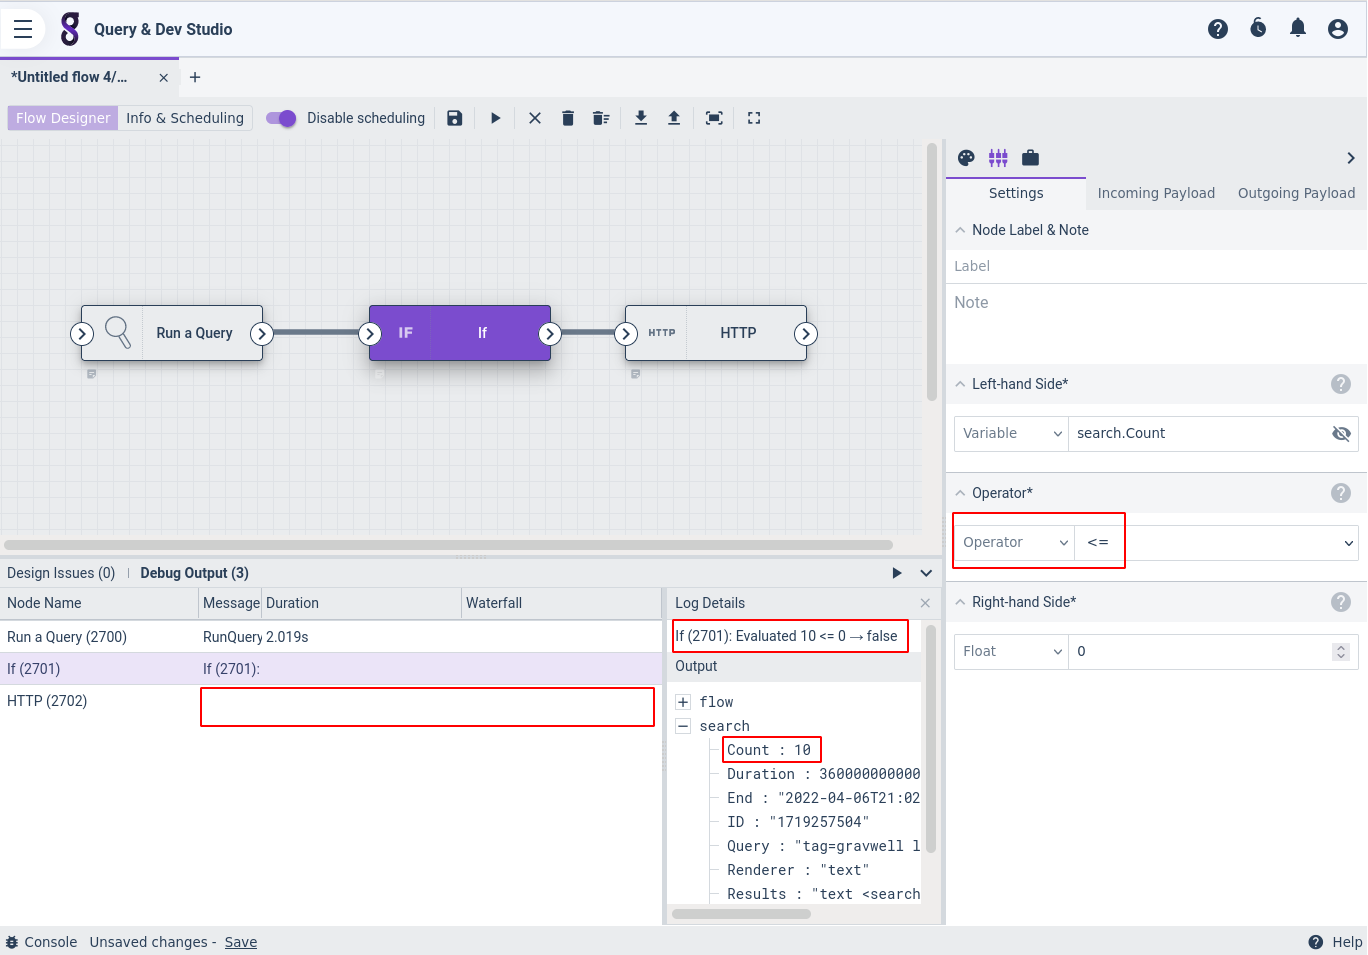
\includegraphics[width=0.85\linewidth]{images/if-false.png}
	\caption{Debug run where If node evaluates to false and execution halts.}
	\label{fig:if-false}
\end{figure}

\subsubsection{Info \& Scheduling}

Once you're happy with a flow, the final step is to give it a schedule and enable it. This is done in the ``Info \& Scheduling'' page, accessible via a button in the toolbar.

You should specify a name and description for the flow, then define a schedule. The schedule is set in cron format\footnote{https://cron.help/}, which is very flexible but can also be intimidating. There are a few shortcuts for simple cases: \code{@hourly} runs at the start of every hour, \code{@daily} at midnight every day, and so on.

\begin{figure}
	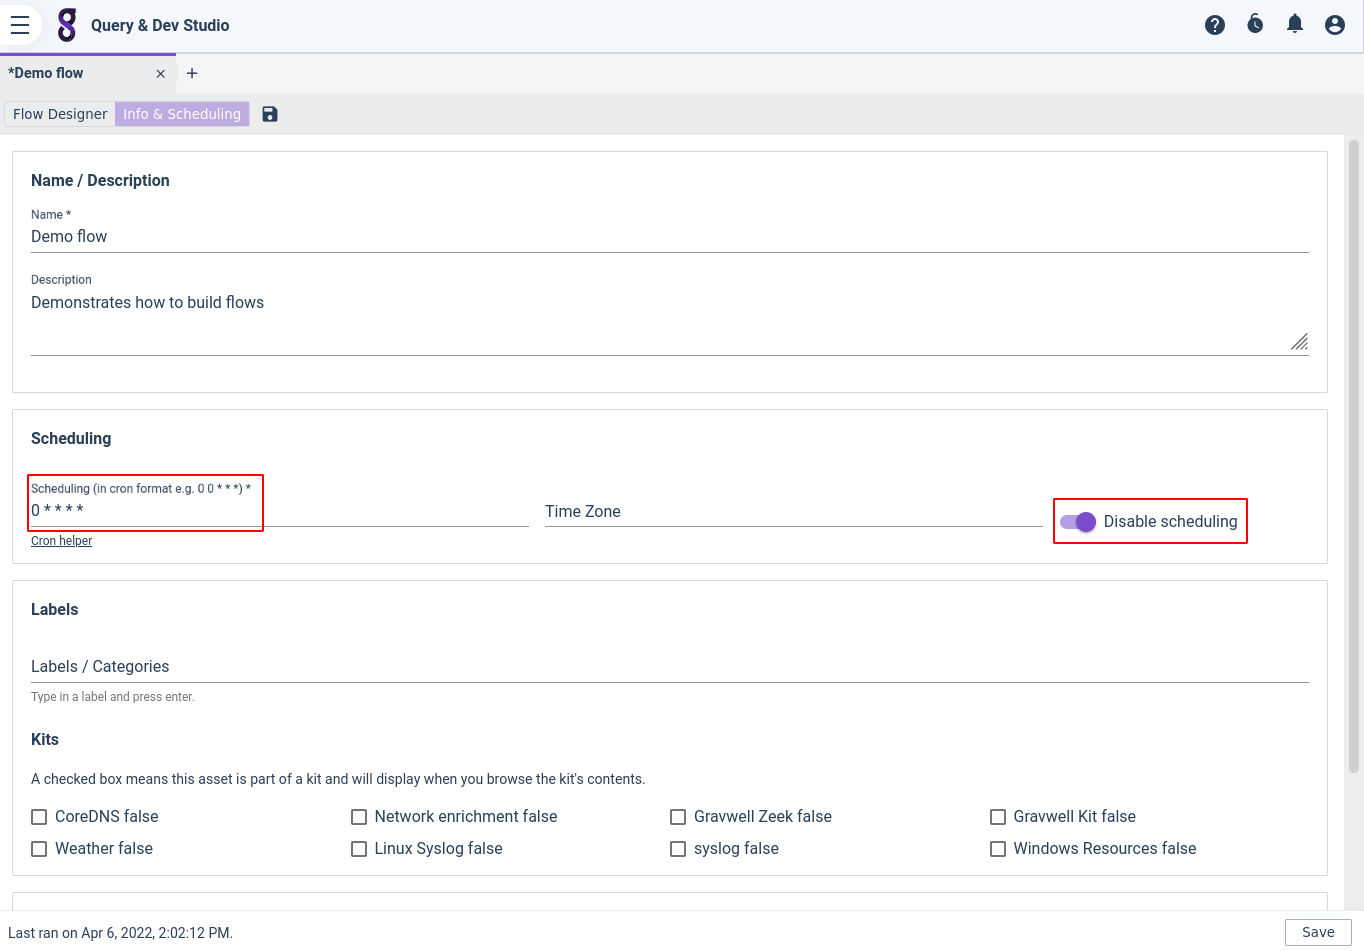
\includegraphics[width=0.85\linewidth]{images/scheduling.png}
	\caption{Info \& scheduling page for flows.}
	\label{fig:scheduling}
\end{figure}

Once the schedule is set, toggle the ``Disable scheduling'' option to enable scheduled executions of the flow. The search agent will then automatically run it on the given schedule.

\subsubsection{In-Flow ``Sticky'' Notes}

The ``Note'' node is a special node used to annotate flows. Unlike other nodes, it plays no role in the execution of the flow; notes exist purely for the convenience of users.

When dragged from the palette, a Note node starts out in a minimized state as seen in Figure \ref{fig:note-minimized}.

\begin{figure}
	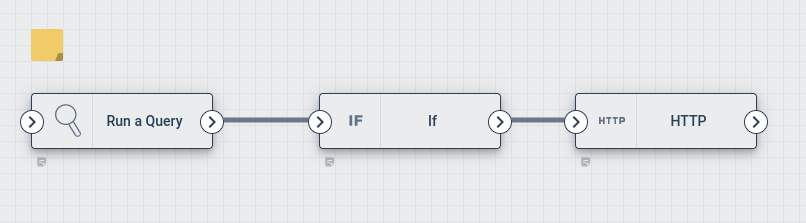
\includegraphics[width=0.6\linewidth]{images/note-minimized.png}
	\caption{A minimized note.}
	\label{fig:note-minimized}
\end{figure}

When clicked, the note expands and text can be entered, as shown in Figure \ref{fig:note-open}.

\begin{figure}
	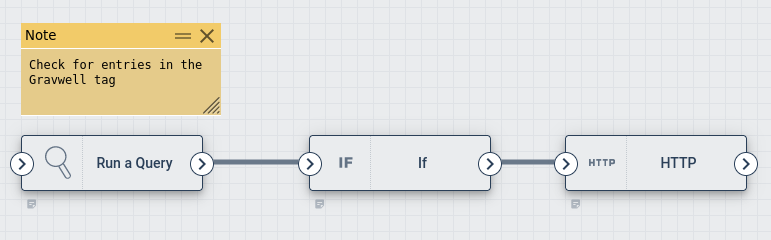
\includegraphics[width=0.6\linewidth]{images/note-open.png}
	\caption{An ``open'' note.}
	\label{fig:note-open}
\end{figure}

Clicking the ``X'' will minimize the note, leaving the start of the text visible as seen in Figure \ref{fig:note-multiple}.

\begin{figure}
	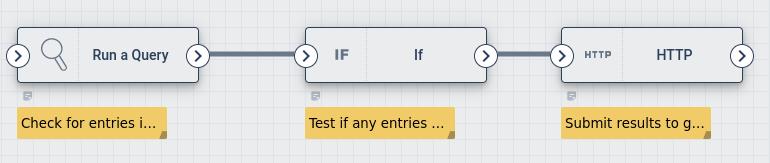
\includegraphics[width=0.6\linewidth]{images/note-multiple.png}
	\caption{Multiple minimized notes with text preview visible.}
	\label{fig:note-multiple}
\end{figure}

\clearpage
\subsection{Nodes}
\label{sec:nodes}

The following nodes are currently implemented:

\begin{itemize}
\item Email: send email messages.
\item Flow Storage Read: read items from a persistent storage.
\item Flow Storage Write: write items into a persistent storage.
\item Gravwell Notification: set Gravwell notifications.
\item HTTP: do HTTP requests.
\item If: perform logical operations.
\item Indexer Info: get information about Gravwell indexers.
\item Ingest: ingest data into Gravwell.
\item Ingester Info: get information about Gravwell ingesters.
\item JavaScript: run small snippets of Javascript code for custom operations.
\item JSON Encode/Decode: encode and decode JSON.
\item Mattermost Message: send a Mattermost message.
\item Nest Merge: join multiple input payloads into one.
\item PDF: create PDF documents.
\item Query Log Ingest: convert search results to alert entries \& ingest.
\item Read Macros: read Gravwell macros.
\item Rename: rename variables in the payload.
\item Run a Query: run a Gravwell query.
\item Set Variables: inject variables into the payload.
\item Slack File: upload a file to a Slack channel.
\item Slack Message: send a message to a Slack channel.
\item Sleep: pause flow execution for a given period of time.
\item Splunk Query: run a Splunk query.
\item Stack Merge: join multiple input payloads into one.
\item Teams Message: send a Microsoft Teams message.
\item Text Template: format text.
\item Throttle: limit execution frequency of certain nodes within a flow.
\end{itemize}

The following nodes tend to be needed only in particular advanced cases:

\begin{itemize}
\item Get Table Results: get results from a search using the table renderer.
\item Get Text Results: get results from a search using the text renderer.
\end{itemize}

A selection of nodes are described in greater detail below. Documentation for every individual node is available on the Gravwell documentation website.\footnote{\href{https://docs.gravwell.io/\#!flows/flows.md}{https://docs.gravwell.io/\#!flows/flows.md}}

\subsubsection{Nest Merge Node}
The Nest Merge node can join multiple input payloads into a single output payload. It ``nests'' each input payload under a different name in the outgoing payload. Figures \ref{fig:nestmerge1} and \ref{fig:nestmerge2} show a simplified example of how this works. Two Set Variable nodes are instantiated, each injecting a variable named ``foo''; the first sets the value to \code{first value} and the other sets the value to \code{second value}. The outputs of these nodes are fed to the Nest Merge node, which has been configured with two input sockets named \code{x1} and \code{x2}. Figure \ref{fig:nestmerge2} shows how the Nest Merge node places the incoming payloads under new top-level names corresponding to the input sockets; thus the \code{foo: "first value"} output of the first Set Variable node is nested under the name \code{x1}.

\begin{figure}
	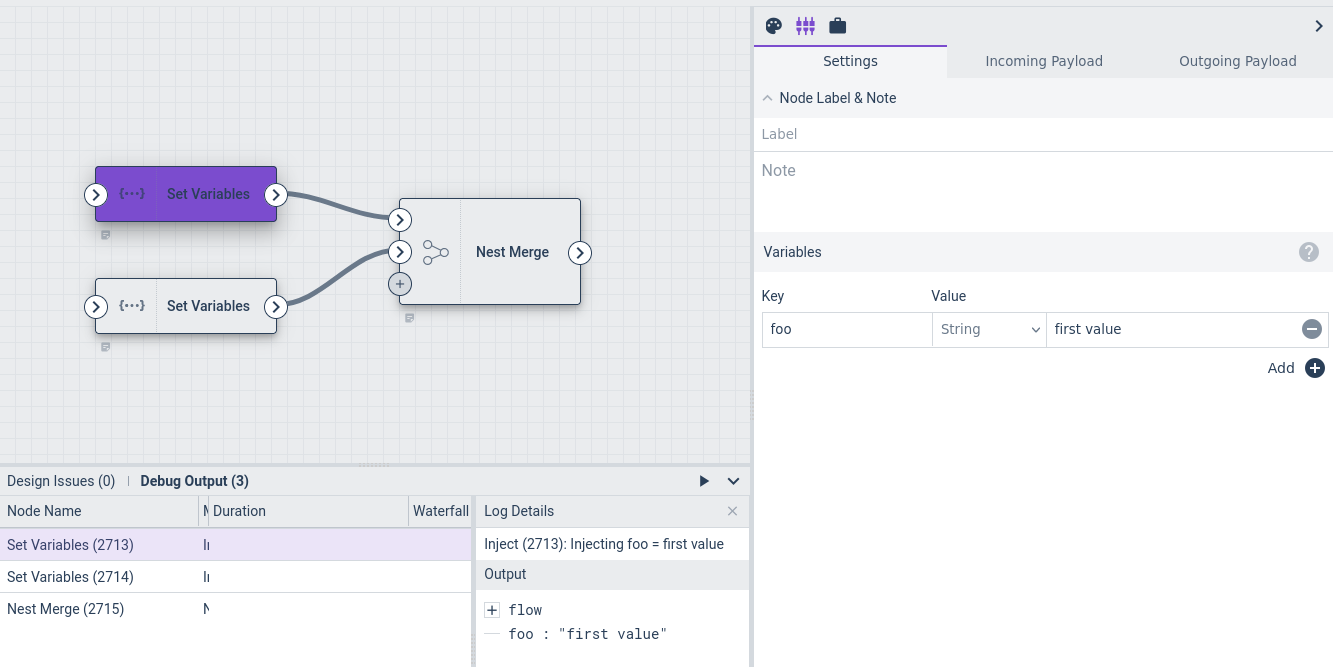
\includegraphics[width=0.85\linewidth]{images/nestmerge1.png}
	\caption{Nest merge inputs.}
	\label{fig:nestmerge1}
\end{figure}

\begin{figure}
	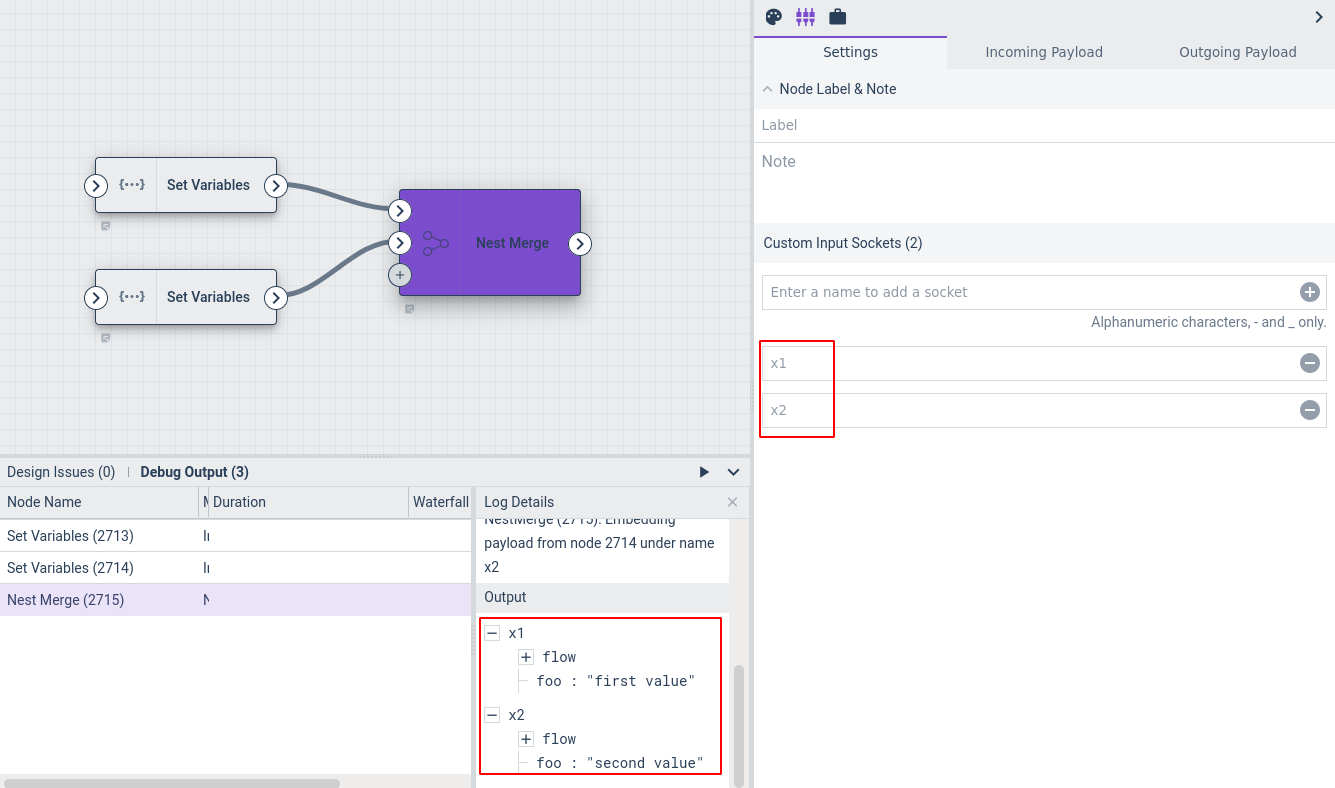
\includegraphics[width=0.85\linewidth]{images/nestmerge2.png}
	\caption{Nest merge output.}
	\label{fig:nestmerge2}
\end{figure}

\subsubsection{Stack Merge Node}
The Stack Merge node can join multiple input payloads into a single output payload. Where the Nest Merge node ``nests'' input payloads and thus always preserves the entirety of all inputs, the Stack Merge node ``overlays'' inputs. That is, it takes the first input payload, then merges in the second payload, \emph{overwriting} any variables with the same name. It repeats this process for all input payloads.

Figures \ref{fig:stackmerge1} and \ref{fig:stackmerge2} show a simplified example of how this works. Two Set Variable nodes are instantiated, each injecting a variable named ``foo''; the first sets the value to \code{first value} and the other sets the value to \code{second value}. The first node also injects a variable named ``x'' with a value of \code{y}.

The outputs of these nodes are fed to the Stack Merge node, which has been configured with two input sockets. Figure \ref{fig:stackmerge2} shows how the Stack Merge node overwrites values; thus the \code{foo: "first value"} output of the first Set Variable node is overwritten by the second node's \code{foo: "second value"} output, but the ``x'' variable is preserved since the second node does not set a variable with the same name.

\begin{figure}
	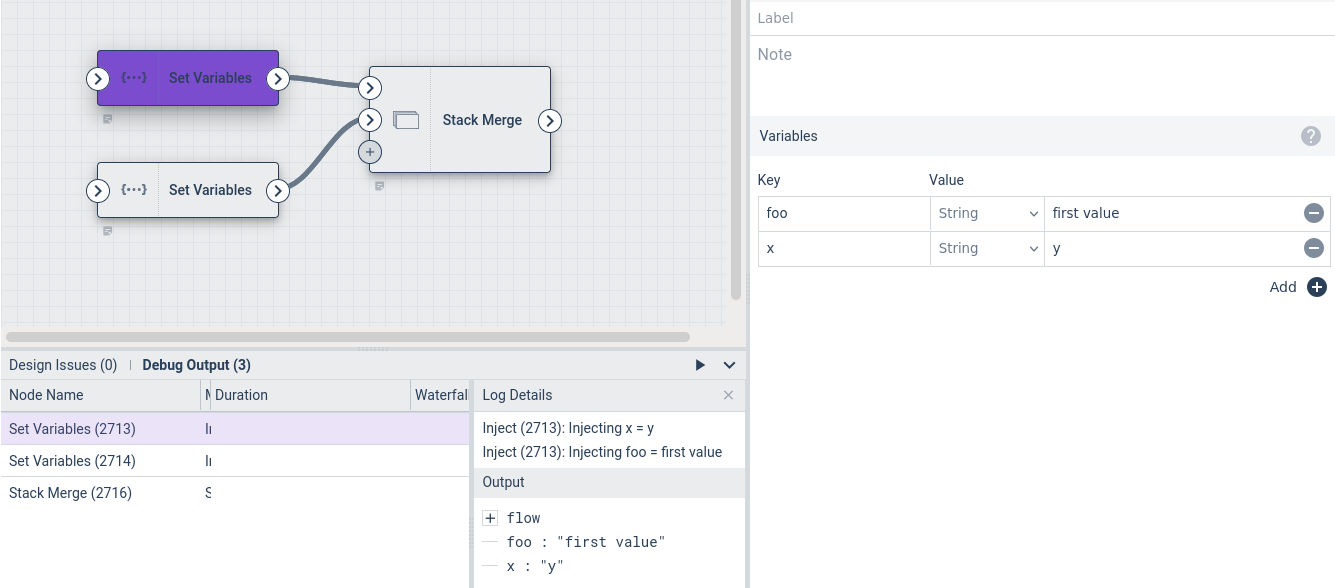
\includegraphics[width=0.85\linewidth]{images/stackmerge1.png}
	\caption{Stack merge inputs.}
	\label{fig:stackmerge1}
\end{figure}

\begin{figure}
	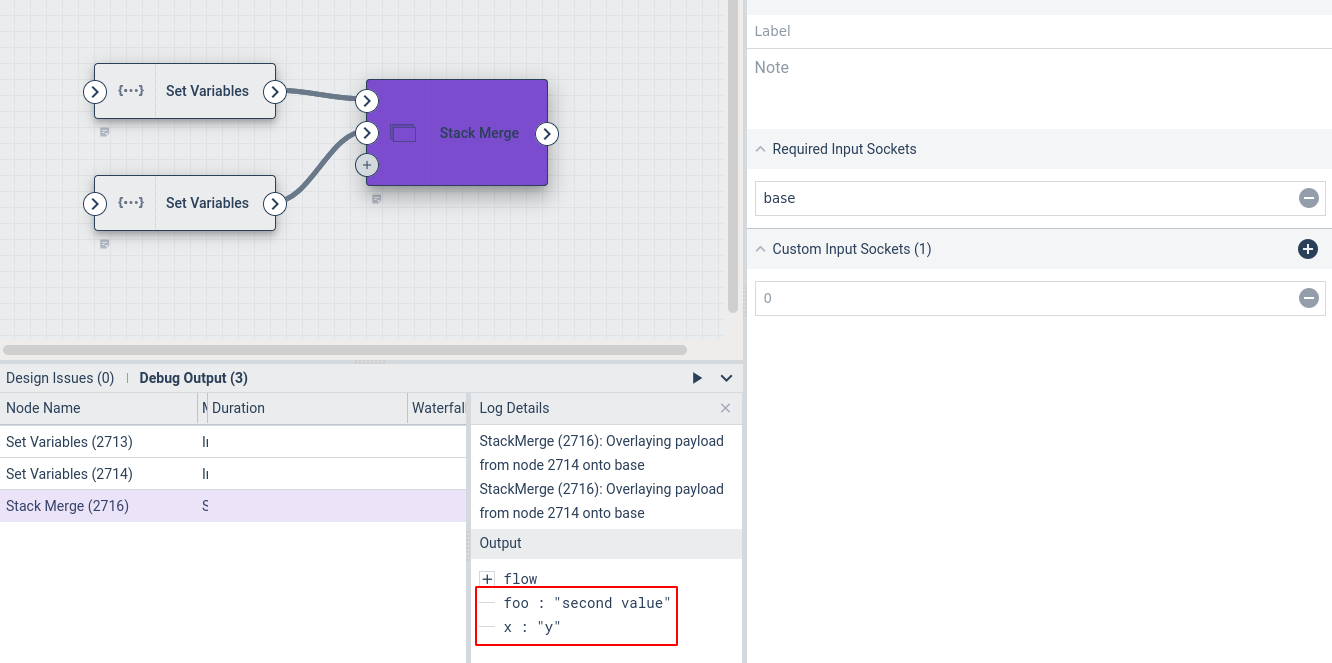
\includegraphics[width=0.85\linewidth]{images/stackmerge2.png}
	\caption{Stack merge output.}
	\label{fig:stackmerge2}
\end{figure}

\subsubsection{Email Node}
The Email node sends emails from within a flow. It can attach items from the payload. Note that the user who owns the flow \emph{must} configure an email server as described in Section \ref{sec:account-menu} for the Email node to function properly!

\begin{itemize}
\item Sender, required: This is the address which will appear in the ``From'' header of the email.
\item Recipients, required: The email will be sent to this address or addresses.
\item Subject, required: The subject line of the email.
\item Body, required: The body text of the email message. Enter a string manually, or select a variable containing suitable text. The Text Template node provides powerful tools for formatting text in the flow.
\item Attachments: An optional array of items to add as attachments on the email.
\end{itemize}

The Email node makes a best-effort attempt at determining the appropriate file type on the attachment. Naming payload items with appropriate file extensions (e.g. appending \code{.pdf} to the output name of the PDF node) helps the Email node figure out the correct type, but it can also make some deductions based on the structure of the data.

\subsubsection{JavaScript Node}
The JavaScript node can execute JavaScript code in a flow, allowing complex logic and custom operations on the payload. The configuration of a JavaScript node consists of three items:

\begin{itemize}
\item Code: the actual JavaScript code to execute.
\item Libraries: a set of libraries to load; these are key-value pairs, where the key is the name of the library (for user reference only) and the value is the content of the library.
\item Outputs: a list of variables to be output from the script (see below).
\end{itemize}

Scripts can read from and write to the payload by accessing the \code{payload} variable, e.g. \code{payload.flow.Scheduled}. Note that variables \emph{created} in the payload are only visible to downstream nodes if that variable is explicitly listed in the ``Outputs'' configuration field.

Combining the HTTP node and the JavaScript node makes it trivially easy to load JS libraries from the Internet. For instance, the flow in Figure \ref{fig:js-flow} uses the HTTP node to fetch the Lodash JavaScript library\footnote{https://raw.githubusercontent.com/lodash/lodash/4.17.15-npm/lodash.js}, then the JavaScript node loads the HTTP response as a library and uses it to round a number. (Note that the Lodash library loads itself into a variable named \code{\_}, so calling the round function from the Lodash library looks like \code{\_.round(4.123)})

\begin{figure}
	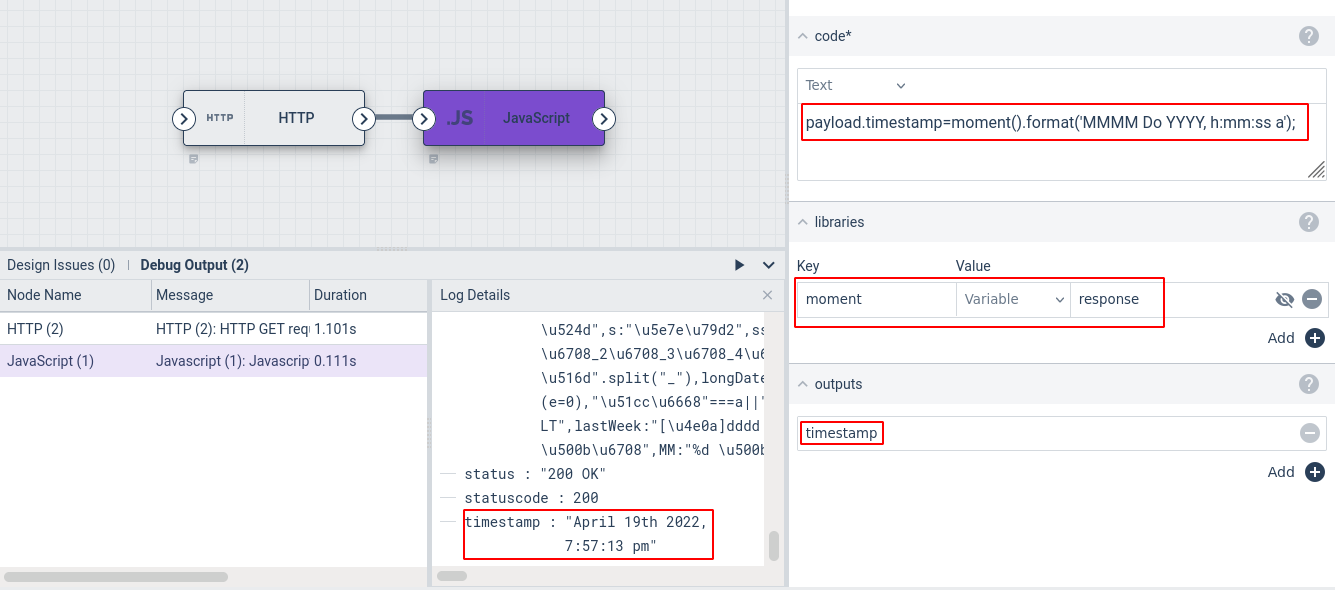
\includegraphics[width=0.85\linewidth]{images/js-flow.png}
	\caption{Loading JavaScript libraries.}
	\label{fig:js-flow}
\end{figure}

\subsubsection{PDF Node}
The PDF node formats search results and other data into an attractive PDF document, which can then be sent to recipients using the Email node, the Slack node, the HTTP node, etc.

There are many configuration options on the PDF node:

\begin{itemize}
\item Title, required: the title of the PDF.
\item Subtitle: an optional sub-title.
\item Contents, required: select one or more items from the payload to be included in the PDF. Query results will be automatically formatted.
\item Page Size: change the size of the pages in the PDF.
\item Include Flow Metadata Page: if set to true, the PDF will include a final page giving information about the execution of the flow.
\item Password: if set, the PDF will be password-protected.
\item Output Variable Name: sets the name for the output PDF in the payload.
\end{itemize}

The ``Contents'' field is perhaps the most critical. The node will attempt to format each item in this field as a section within the PDF document. It knows how to parse query results, meaning that a query using the table renderer will be inserted into the PDF as a proper table. Figure \ref{fig:pdf-contents} shows an example flow in which the outputs of several queries, plus the output of a Text Template node, are used as the Contents of a PDF. Figure \ref{fig:pdf-result} shows an example of what such a PDF may look like.

\begin{figure}
	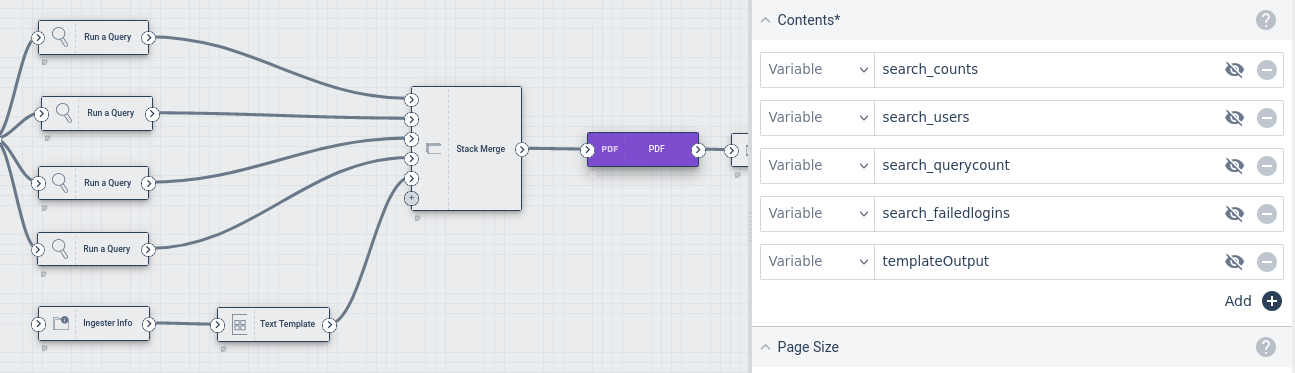
\includegraphics[width=0.95\linewidth]{images/pdf-contents.png}
	\caption{Including multiple query results in a PDF.}
	\label{fig:pdf-contents}
\end{figure}

\begin{figure}
	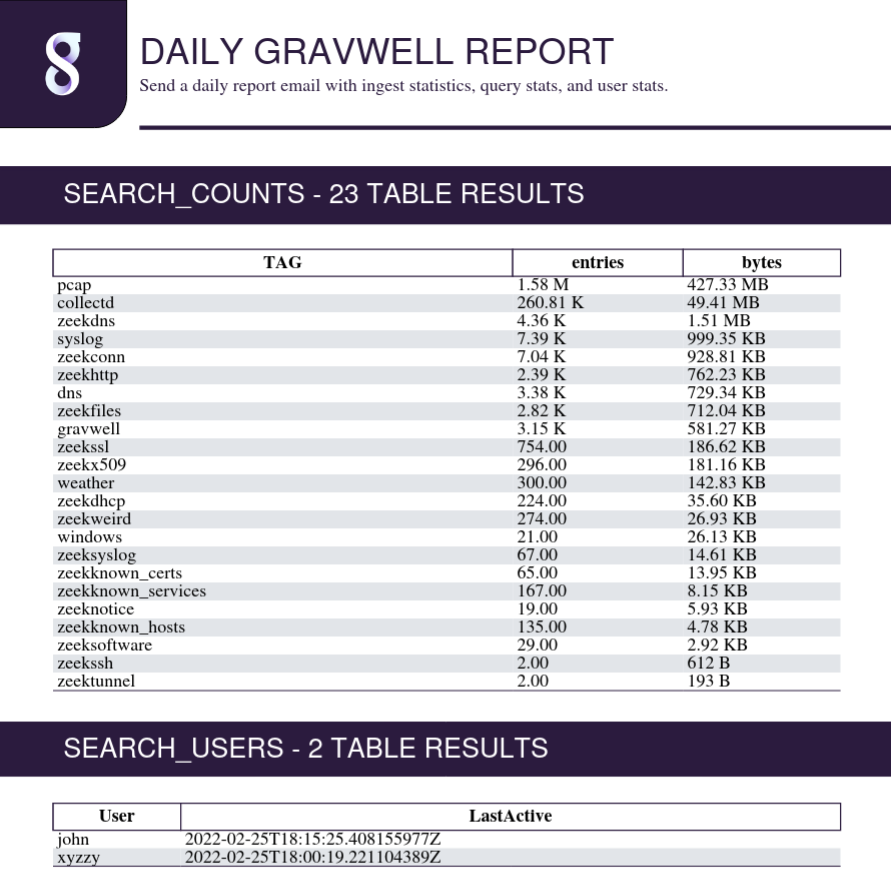
\includegraphics[width=0.85\linewidth]{images/pdf-result.png}
	\caption{Sample PDF output.}
	\label{fig:pdf-result}
\end{figure}

The ``Output Variable Name'' config option specifies the name to use for the output PDF in the payload. Using a name which ends in \code{.pdf} will help inform other nodes that the object is a PDF file, for instance when included as an attachment on the Email node.

Setting ``Include Flow Metadata Page'' to true causes the node to insert an additional page at the end of the document containing additional information about the user who executed the flow, the status of the Gravwell cluster, and the current Gravwell license. It will also insert the full query string, the timeframe, and the execution time for any queries which were packaged into the PDF.
\clearpage

\subsubsection{Slack File/Message Nodes}
Two nodes can send to Slack: Slack Message and Slack File. As the names imply, one sends a text message to a Slack channel, while the other uploads a file. Both nodes have the following configuration options:

\begin{itemize}
\item Token, required: a Slack access token\footnote{\href{https://api.slack.com/authentication/token-types}{https://api.slack.com/authentication/token-types}} for the desired server.
\item Channel, required: the channel that will receive the message, \emph{without} a preceding `\#' character.
\item Message: the message body; Markdown is supported.
\end{itemize}

The Slack Message node also has a ``Verbatim Text'' config, which is optional text to be attached to the message verbatim, without being parsed as Markdown. This is useful for showing the result of an HTTP request or other unformatted data.

The Slack File node also has a ``File to Send'' config, which is an item from the payload to be attached to the message. This works particularly well with the output of the PDF node.

Note that any user with read access to the flow will be able to extract the token, giving them the ability to write to the same Slack server. For this reason, we recommend that flows with Slack nodes should not be shared with other users.

\subsubsection{Teams Node}
The Teams node can send a message to a Microsoft Teams channel. The configuration options are:

\begin{itemize}
\item Webhook, required: an incoming webhook\footnote{\href{https://docs.microsoft.com/en-us/microsoftteams/platform/webhooks-and-connectors/what-are-webhooks-and-connectors}{https://docs.microsoft.com/en-us/microsoftteams/platform/webhooks-and-connectors/what-are-webhooks-and-connectors}} URL for Microsoft Teams.
\item Title: an optional title for the message.
\item Message, required: the body of the message to send.
\end{itemize}

Note that any user with read access to the flow will be able to extract the webhook, giving them the ability to write to the same Teams channel. For this reason, we recommend that flows with Teams nodes should not be shared with other users.

\clearpage
\subsection{Hands-On Lab: Flows}
\label{sec:flow-lab}
This lab will demonstrate how to build a flow. The flow will send a notification whenever there have been failed login attempts to the Gravwell system. First, create a Gravwell webserver+indexer container:

\begin{Verbatim}[breaklines=true]
docker run -d --rm --net gravnet -p 8080:80 --name gravwell gravwell:base
\end{Verbatim}

Now log into the web GUI (\href{http://localhost:8080}{http://localhost:8080}). After that, open a new \emph{private} browser window (so the existing login cookie isn't used) and enter some invalid login credentials, e.g. username ``admin'' with password ``admin''. This will generate a login failure message which we can check using the following query:

\begin{Verbatim}[breaklines=true]
tag=gravwell syslog Message=="Authentication failure" user 
| stats count by user 
| table user count
\end{Verbatim}

\begin{figure}
	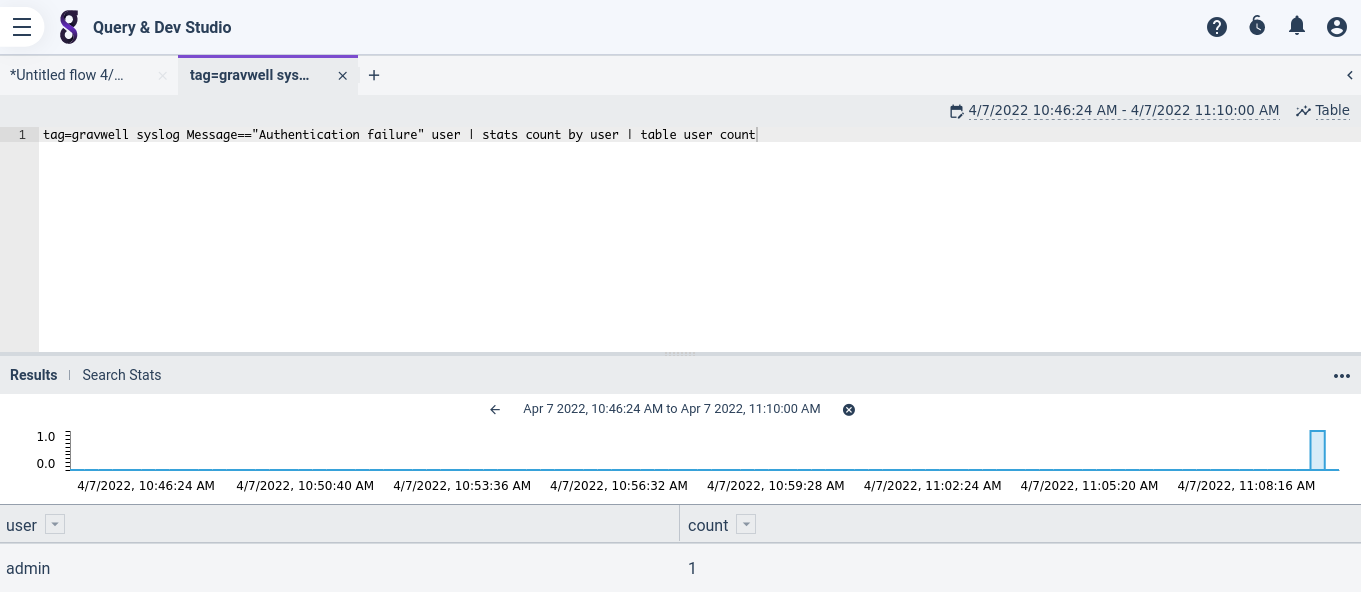
\includegraphics[width=0.85\linewidth]{images/lab-failed-logins.png}
	\caption{Query showing failed login attempts.}
	\label{fig:lab-failed-logins}
\end{figure}

We will use that query as the basis for a new flow. Select ``Flows'' from the ``Automation \& Flows'' section in the main menu, then click the ``+'' icon in the upper right to create a new flow. Drag the following nodes from the node palette out to the canvas:

\begin{itemize}
\item Run a Query
\item If
\item Gravwell Notification
\end{itemize}

Wire them up as seen in Figure \ref{fig:lab-nodes}

\begin{figure}
	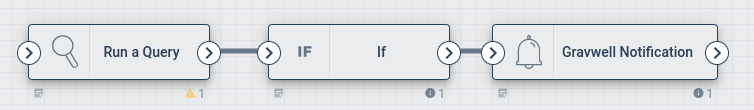
\includegraphics[width=0.7\linewidth]{images/lab-nodes.png}
	\caption{Node layout for lab.}
	\label{fig:lab-nodes}
\end{figure}

Each node now needs to be configured. Begin with the Run a Query node; click it, then paste the Gravwell query above into the ``Query String'' config field. Note how the ``Search Timeframe'' defaults to the last hour, and ``Output Variable Name'' defaults to ``search''. This means the payload output by the Run a Query node will contain an item named ``search'' with information about the query which was executed.

The If node should be configured to check \code{search.Count > 0}. This means that execution will continue if there were any results from the search.

Finally, set a message in the Gravwell Notification node's Message field, something like ``Failed logins! Go check!''.

Once all three nodes are configured, the Design Issues tab of the console should be empty. If there are issues reported, check your configuration on the associated node.

To test the flow, click the debug icon in the toolbar. You should soon see a notification appear as in Figure \ref{fig:lab-notification}.

\begin{figure}
	
\includegraphics[width=0.7\linewidth]{images/lab-notification.png}
	\caption{Example notification from flow.}
	\label{fig:lab-notification}
\end{figure}

If no notification appears, double-check that the query given above actually returns results when run over the last hour, or try generating more failed login attempts.

Once the flow is working, you can prepare the flow for deployment.  In the Run Query node's config, change the Search Timeframe dropdown from ``ISO Duration'' to ``Variable''. The value should change to the default \code{flow.Interval}. Then go to the Info \& Scheduling tab, set the schedule to ``* * * * *'' to make it run every minute, toggle the ``Disable scheduling'' slider, and hit Save. These two changes will make the flow run automatically every minute, and cause the query to run only over the last minute (this is the effect of setting the duration to \code{flow.Interval}).

Test these changes by periodically creating failed login events. You should see a notification pop up after a failed login. Delete the notification; it should not come back again until you do another failed login.

To clean up after the experiment, run:

\code{docker kill \$(docker ps -a -q)}
